\documentclass[a4paper, 12pt, twoside, openright]{article}
\usepackage[T1]{polski}
\usepackage[utf8]{inputenc}
\newtheorem{theorem}{Twierdzenie}
\usepackage{helvet}
\usepackage{graphicx}
\usepackage{color}
\usepackage{subfig}
\usepackage[table, svgnames, dvipsnames]{xcolor} 
\usepackage{array}
\usepackage{float}
\usepackage{cellspace}
\usepackage[top=1.3in,bottom=1.3in,right=1in,left=1in,headheight=95pt,headsep=-0.5cm]{geometry}
\usepackage{color}
\usepackage{listings}
\usepackage{caption}
\usepackage{cmap}

\usepackage{enumitem}
\setlist{nolistsep}
\usepackage{hyperref}
\usepackage{listings}

\definecolor{mGreen}{rgb}{0,0.6,0}
\definecolor{mGray}{rgb}{0.5,0.5,0.5}
\definecolor{mPurple}{rgb}{0.58,0,0.82}
\definecolor{backgroundColour}{rgb}{0.95,0.95,0.92}

\lstdefinestyle{CStyle}{
    backgroundcolor=\color{backgroundColour},
    commentstyle=\color{mGreen},
    keywordstyle=\color{magenta},
    numberstyle=\tiny\color{mGray},
    stringstyle=\color{mPurple},
    basicstyle=\footnotesize,
    breakatwhitespace=false,
    breaklines=true,
    captionpos=b,
    keepspaces=true,
    numbers=left,
    numbersep=5pt,
    showspaces=false,
    showstringspaces=false,
    showtabs=false,
    tabsize=2,
    language=C
}

\lstdefinestyle{CStyleLine}{
    backgroundcolor=\color{backgroundColour},
    commentstyle=\color{mGreen},
    keywordstyle=\color{magenta},
    numberstyle=\tiny\color{mGray},
    stringstyle=\color{mPurple},
    basicstyle=\footnotesize,
    breakatwhitespace=false,
    breaklines=true,
    captionpos=b,
    keepspaces=true,
    numbersep=5pt,
    showspaces=false,
    showstringspaces=false,
    showtabs=false,
    tabsize=2,
    language=C
}


\newcounter{nalg} 
\DeclareCaptionLabelFormat{algocaption}{Algorytm \thenalg}
\lstnewenvironment{algorithm}[1][] 
{   
	\refstepcounter{nalg}
	\captionsetup{labelformat=algocaption,labelsep=colon} 
	\lstset{ 
		mathescape=true,
		frame=tB,
		numbers=left, 
		numberstyle=\tiny,
		basicstyle=\scriptsize, 
		keywordstyle=\color{black}\bfseries\em,
		keywords={,input, def, output, return, datatype, function, in, if, else, foreach, while, begin, end }
		numbers=left,
		xleftmargin=.04\textwidth,
		#1 
	}
}
{}



\begin{document}

\lstset{language=Python}
% =====  STRONA TYTULOWA  ====

\thispagestyle{empty}
\vspace*{-0.6in}
%% ------------------------ NAGLOWEK STRONY =======================------

\includegraphics[height=37.5mm]{img/logo_agh}\\
\rule{30mm}{0pt}
{\large\textsf{Wydział Fizyki i Informatyki Stosowanej}}\\
\rule{\textwidth}{3pt}\\
\rule[2ex]
{\textwidth}{1pt}\\
\vspace{3ex}
\begin{center}
{\bf\LARGE\textsf{Praca inżynierska}}\\
\vspace{13ex}
% ======================= IMIE I NAZWISKO =======================----
{\bf\Large\textsf{Patryk Chodur}}\\
\vspace{3ex}
{\sf \small kierunek studiów:} {\bf\small\textsf{informatyka stosowana}}\\
\vspace{15ex}
%% ------------------------ TYTUL PRACY --------------------------------------
{\bf\huge\textsf{Opracowanie wtyczki do dekodowania
	pakietów Ethernet z~wykorzystaniem oprogramowania Wireshark
}}\\
\vspace{14ex}
%% ------------------------ OPIEKUN PRACY ------------------------------------
{\sf \Large Opiekun:} {\bf\Large\textsf{dr hab. inż. Bartosz Mindur}}\\
\vspace{22ex}
\textsf{\bf\large\textsf{Kraków, styczeń 2021}}
\end{center}


\newpage

%% =====  Oświadczenie =========
\begin{center}
	{\bf\large\textsf{Oświadczenie studenta}}
\end{center}


{\sf Uprzedzony(-a) o odpowiedzialności karnej na podstawie art. 115 ust. 1 i 2 ustawy z dnia 4 lutego 1994 r. o prawie autorskim i prawach pokrewnych (t.j. Dz. U. z 2018 r. poz. 1191 z późn. zm.): „Kto przywłaszcza sobie autorstwo albo wprowadza w błąd co do autorstwa całości lub części cudzego utworu albo artystycznego wykonania, podlega grzywnie, karze  ograniczenia wolności albo pozbawienia wolności do lat 3. Tej samej karze podlega, kto rozpowszechnia bez podania nazwiska lub pseudonimu twórcy cudzy utwór w wersji oryginalnej albo w postaci opracowania, artystyczne wykonanie albo publicznie zniekształca taki utwór, artystyczne wykonanie, fonogram, wideogram lub nadanie.”, a także uprzedzony(-a) o odpowiedzialności dyscyplinarnej na podstawie art. 307 ust. 1 ustawy z dnia 20 lipca 2018 r. Prawo o szkolnictwie wyższym i nauce (Dz. U. z 2018 r. poz. 1668 z późn. zm.) „Student podlega odpowiedzialności dyscyplinarnej za naruszenie przepisów obowiązujących w uczelni oraz za czyn uchybiający godności studenta.”, oświadczam, że niniejszą pracę dyplomową wykonałem(-am) osobiście i samodzielnie i nie korzystałem(-am) ze źródeł innych niż wymienione w pracy

\bigskip

Jednocześnie Uczelnia informuje, że zgodnie z art. 15a ww. ustawy o prawie autorskim i prawach pokrewnych Uczelni przysługuje pierwszeństwo w opublikowaniu pracy dyplomowej studenta. Jeżeli Uczelnia nie opublikowała pracy dyplomowej w terminie 6 miesięcy od dnia jej obrony, autor może ją opublikować, chyba że praca jest częścią utworu zbiorowego. Ponadto Uczelnia jako podmiot, o którym mowa w art. 7 ust. 1 pkt 1 ustawy z dnia 20 lipca 2018 r. — Prawo o szkolnictwie wyższym i nauce (Dz. U. z 2018 r. poz. 1668 z późn. zm.), może korzystać bez wynagrodzenia i bez konieczności uzyskania zgody autora z utworu stworzonego przez studenta w wyniku wykonywania obowiązków związanych z odbywaniem studiów, udostępniać utwór ministrowi właściwemu do spraw szkolnictwa wyższego i nauki oraz korzystać z utworów znajdujących się w prowadzonych przez niego bazach danych, w celu sprawdzania z wykorzystaniem systemu antyplagiatowego. Minister właściwy do spraw szkolnictwa wyższego i nauki może korzystać z prac dyplomowych znajdujących się w prowadzonych przez niego bazach danych w zakresie niezbędnym do zapewnienia prawidłowego utrzymania i rozwoju tych baz oraz współpracujących z nimi systemów informatycznych.}

\vspace{14ex}

\begin{center}

~~~~~~~~~~~~~~~~~~~~~~~~~~~~~~~~~~~~~~~~~~~~~~~~~~~~~~~~~~~~~~~~~ 
................................................................. \\
~~~~~~~~~~~~~~~~~~~~~~~~~~~~~~~~~~~~~~~~~~~~~~~~~~~~~~~~~~~~~~~  {\sf (czytelny podpis)} \\

\end{center}

%% =====  TYL STRONY TYTULOWEJ   ====


%% ============ OCENA OPIEKUNA =============
\newpage
\linespread{1.3}
\selectfont

\hspace*{\fill}\large{Ocena merytoryczna opiekuna}

\vspace{85mm}

%% ============ OCENA RECENZENTA =============
\newpage
\linespread{1.3}
\selectfont

\hspace*{\fill}\large{Ocena merytoryczna recenzenta}

\vspace{85mm}


%% ====== SPIS TRESCI ==========
\newpage
\tableofcontents


%=======================- 1 =======================
\newpage
\section{Wstęp}

	\subsection{Wprowadzenie}
	\indent\par
	Sniffer to program komputerowy, którego celem jest przechwytywanie i monitorowanie ruchu internetowego. Umożliwia on
	podglądanie pakietów w celu ich analizy pod kątem zawartości, rozmiaru, zastosowania, czy celu. Powodów do takiej
	analizy jest wiele. Użytkownik może chcieć badać komunikację dwóch urządzeń będących częścią autorskiego systemu
	informatycznego, sprawdzać zajętość łącza internetowego, debugować własną aplikację korzystającą z sieci, czy podglądać
	ruch internetowy innego użytkownika.

	Na rynku dostępnych jest wiele narzędzi przeznaczonych do tego celu, różniących się funkcjonalnością, ceną czy licencją.
	Najpopularniejsze z nich to:
	\begin{itemize}
		\item \texttt{tcpdump} - jeden z pierwszych snifferów, dostępny za darmo na 3-klauzulowej licencji BSD. Działa
			z większością systemów opartych na Unixie, bądź nim inspirowanych. Do obsługi używany jest wiersz poleceń.
		\item \texttt{WinDump} - port tcpdump na platformę Windows, udostępniony na tej samej licencji.
		\item \texttt{Wireshark} - darmowy i otwarty program do analizy ruchu internetowego. Wyposażony jest on w graficzny
			interfejs i stanowi prostszą w obsłudze alternatywę dla \texttt{tcpdump}. Jest on wykorzystany zarówno w reszcie
			wstępu, jak i całej pracy. Udostępniony na licencji GPLv2.
	\end{itemize}

	Dostępnych jest więcej narzędzi, w tym płatne, lecz popularność powyższych jest sprawia, że nie ma konieczności wpominiania
	reszty.

	Jedną z podstawowych funkcjonalności snifferów jest podglądanie zawartości przechodzących przez łącze internetowe danych.
	Dokonuje się tego za pomocą dekoderów (ang. dissector). 

	\newpage
	\subsubsection{Dekodery}
	\indent\par
	Dekoder to część sniffera zajmująca się rozkodowywaniem pakietów określonego typu. Rozkodowywanie polega na intepretacji
	ciągu bajtów, jakim jest pakiet, i wyciąganiu z niego użytecznych informacji. Umiejscowienie danych, i ich znaczenie,
	charakterystyczne jest dla danego typu pakietu. Aby rozkodowywać różne pakiety potrzebny jest więc zbiór dekoderów. 

	Pakiet może przenosić dane innego typu, które także wymagają rozkodowania. Dekodery mają więc strukturę hierarchiczną -
	wyjście jednego może stanowić wejście drugiego dekodera.

	\begin{figure}[ht]
		\centering
			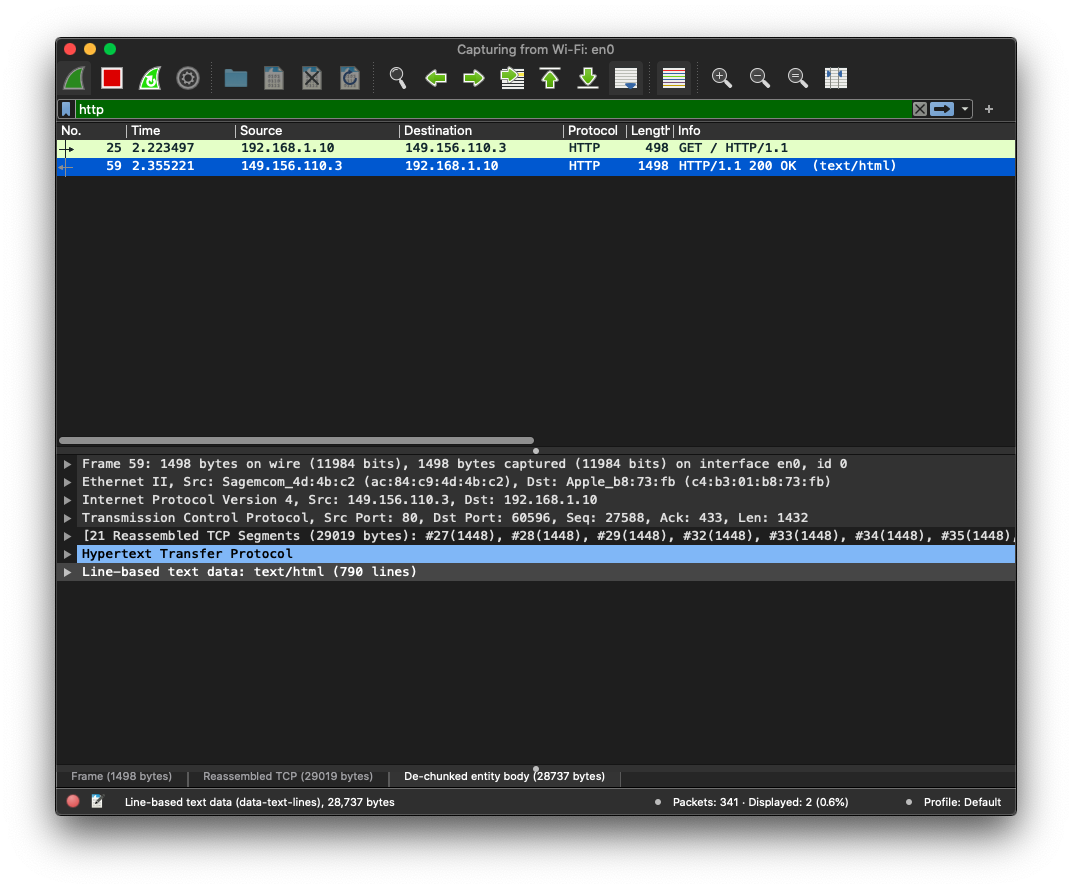
\includegraphics[width=1.0\textwidth]{img/screenshot_fis.png}
		\caption{Przykładowa struktura pakietu http po wyświetleniu w przeglądarce strony http://www.fis.agh.edu.pl}
		\label{fig:fis}
	\end{figure}

	Na powyższym rysunku (Rys.~\ref{fig:fis}) widać kolejne poziomy dekodowania pakietu http. Są to:

	\begin{itemize}
		\item Interfejs en0
		\item Protokół Ethernet
		\item Protokół IPv4
		\item Protokół TCP
		\item Dodatkowy poziom złożonych pakietów TCP
		\item Protokół http
		\item Dane tekstowe
	\end{itemize}

	Każdy dekoder jest osobnym modułem, dzięki czemu np. dekoder http może czytać także dane idące protokołem UDP.
	Dekodery rejestrują zainteresowanie danymi pakietami dekoderowi wyżej w hierarchii, więc dekoder http może przykładowo
	żądać danych przesyłanych protokołem TCP na porcie 80. Istnieją także dekodery heurystyczne, cechujące się brakiem
	konieczności podawania konkretnych parametrów dekoderowi wyżej w hierarchii, oraz możliwością odrzucenia pakietu,
	aby mógł zostać użyty przez inny dekoder, zostaną jednak one celowo, ze względu na znaczną złożoność i brak bezpośredniego
	związku z pracą, pominięte.

	Głównym zadaniem dekoderów jest wyświetlanie przesyłanych informacji w sposób zrozumiały dla użytkownika. Za pomocą
	interfejsu graficznego wyświetlają one zinterpretowane przez siebie dane transmisji. Sposób przedstawienia danych
	jest arbitralną decyzją programisty, więc podstawowymi kryteriami podczas projektowania są użyteczność oraz czytelność.

	\begin{figure}[ht]
		\centering
			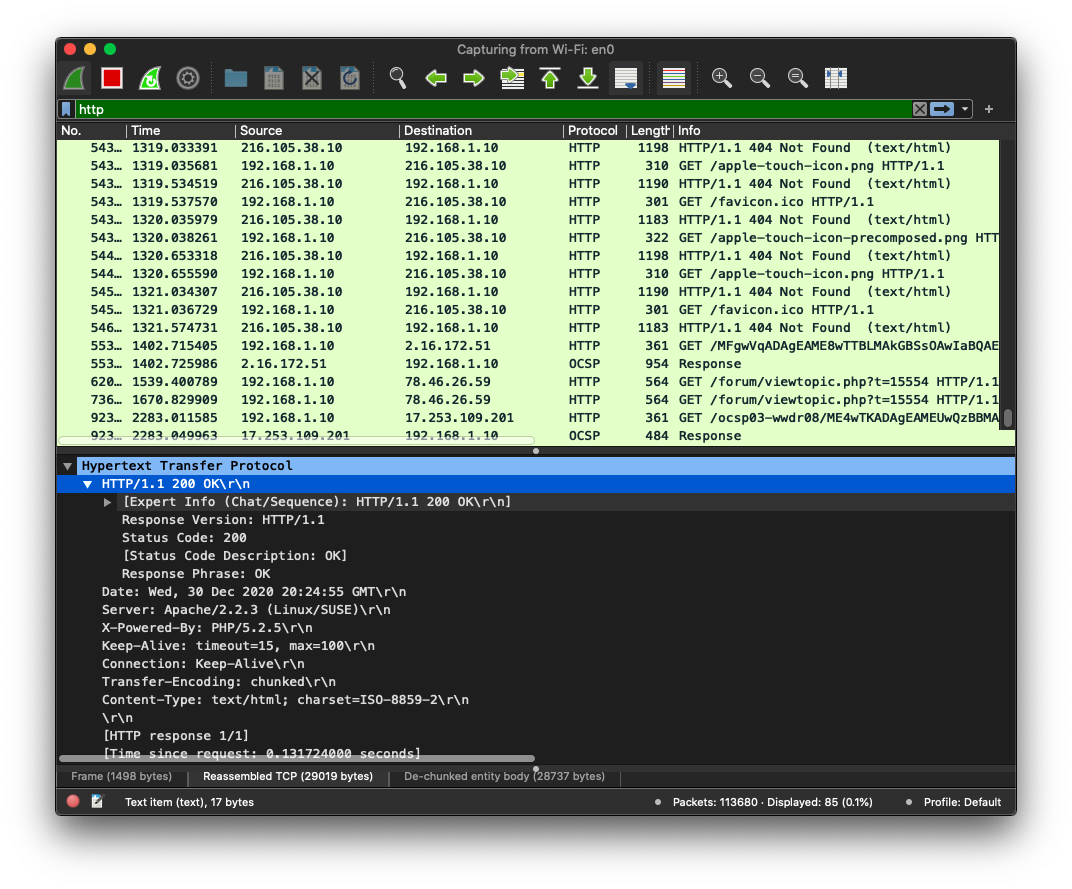
\includegraphics[width=1.0\textwidth]{img/screenshot_fis_http.png}
		\caption{Binarne dane protokołu http zinterpretowane przez odpowiedni dekoder i wyświetlone w oknie programu.}
		\label{fig:fis_http}
	\end{figure}

	\newpage
	\subsubsection{Tworzenie dekoderów}
	\indent\par
	Program Wireshark wyposażony jest w zestaw dekoderów do najczęściej wykorzystywanych protokołów. Twórcy programu
	dają jednakże możliwość tworzenia własnych. Głównym celem ich tworzenia jest możliwość
	dekodowania własnych protokołów oraz reintepretacja już istniejących. Dostępne są trzy sposoby ich pisania:
	\begin{itemize}
		\item Tekstowe - opisana w formie tekstowej struktura pakietu oraz inne, konieczne do zdekodowania informacje.
		\item Skryptowe - dekoder napisany w języku skryptowym, np. \texttt{lua} czy \texttt{python}
		\item Kompilowane, w języku C - dekoder napisany jako kompilowana wtyczka w C
	\end{itemize}

	Tekstowe dekodery są najprostsze w implementacji, jednak działają zwykle najwolniej, a ich możliwości są ograniczone.
	Dekodery napisane w C mają największe możliwości, gdyż mogą chociażby korzystać z \texttt{libwireshark}. Działają zwykle
	najszybciej, a gotowy plugin łatwo jest przenieść do innej instalacji, ale ich problemem jest wyższy próg wejścia. 
	Są też najobszerniejsze i najmniej czytelne.

	Kompromis pomiędzy tymi dwoma podejściami stanowi pisanie w języku skryptowym. Najczęściej wykorzystywany w tym celu jest
	język \texttt{lua}. Cieszy się on wbudowanym wsparciem ze strony programu Wireshark oraz stosunkowo dużą społecznością.



	\newpage
\subsection{Cel pracy}

	\indent\par
	Celem pracy jest wykonanie dekodera pakietów bazujących na protokole UDP i~przenoszących konkretne dane pomiarowe.
	Dekoder napisany jest jako wtyczka do programu Wireshark. Podejście takie umożliwia szybszą rekompilację wtyczki,
	niewymagającą przekomilowywania całego programu, a~także użycie gotowej wtyczki z~dowolną instalacją programu Wireshark,
	o~ile zachowana jest zgodność systemu operacyjnego i~wersji programu Wireshark. Instalacja polega na przekopiowaniu
	pojedyńczego pliku do katalogu wtyczek programu. Alternatywą dla takiego rozwiązania jest stworzenie wbudowanego dekodera,
	ale ze względu na liczne wady - m.~in.: dłuższy czas rekompilacji oraz konieczność ingerencji w~kod źródłowy programu - rozwiązanie
	to nie zostało zastosowane.

	Przechwytywane dane pochodzą z urządzenia GEMROC ASIC. Każdy pakiet ma stałą długość (1500 bajtów) i przekazywany jest 
	protokołem UDP na porcie 48350. Struktura pakietu jest następująca:
	\begin{itemize}
		\item Pierwsze 8 bajtów transmisji to numer pakietu.
		\item Kolejne 8 bajtów to status.
		\item Dalej przesyłane są dane w formie 8 bajtowych pól bitowych.
		\item Ostatnie 2 bajty to ilość danych.
	\end{itemize}

	Status jest jeden dla całego pakietu i zawiera pola:
	\begin{itemize}
		\item Clk state
		\item I2C status
		\item ADC Clk sel
		\item ASIC enable status
	\end{itemize}

	Dane składają się z pól:
	\begin{itemize}
		\item ADC
		\item Timestamp FPGA
		\item Timestamp ASIC
		\item Channel ID
		\item ASIC ID
		\item PileUp
		\item Overflow
	\end{itemize}



\newpage
\section{Narzędzia}
\subsection{Kod źródłowy}

	\indent\par
	Wtyczka napisana została w języku C, bez jawnego użycia zewnętrznych bibliotek. Wykorzystane pliki nagłówkowe
	pochodzą ze standardowej biblioteki C, oraz kodu źródłowego programu Wireshark - w szczególności \texttt{libwireshark}.
	Program Wireshark używa wielu bibliotek, takich jak \texttt{qt} oraz \texttt{gthread}, ale na wyszczególnienie zasługuje biblioteka
	\texttt{glib} w wersji drugiej, której
	elementy zostały użyte w kodzie źródłowym aplikacji. \texttt{Glib2} dostarcza projektowi standardowych typów o stałym
	rozmiarze wykorzystywanych przez niektóre funkcje Wireshark.
	
	Cały kodu projektu napisany został w programie Vim.

\subsection{Kompilacja}

	\indent\par
	Podczas kompilacji projektu wykorzystywane jest narzędzie cmake. Służy ono do zarządzania procesem kompilacji,
	umożliwiając jednolity proces budowy projektu
	na każdym ze wspieranych systemów operacyjnych. Wykrywa ono konieczne do zbudowania narzędzia, informując
	o brakujących, a także, w zależności od systemu operacyjnego, tworzy skrypty kompilacyjne. Na systemach Unixowych
	oznacza to zwykle generowanie plików Makefile, na systemie Windows - projektu w Visual Studio. Użycie cmake'a
	jest pierwszym krokiem standardowej kompilacji programu Wireshark oraz jego wtyczek.
	
	Do kompilacji wymagany jest kompilator do języka C. Decyzję o wykorzystaniu konkretnego narzędzia podejmuje cmake.
	W razie braku stosownego kompilatora cmake poinformuje użytkownika o problemie. Ponadto wymagany jest szereg
	bibliotek.

	\newpage

	Część wymagań dla Wireshark 3.4.2:
	\begin{itemize}
		\item \texttt{GLIB2} - biblioteka od GNU będąca implementacją biblioteki standardowej C wraz z wieloma rozszerzeniami.
		\item \texttt{GTHREAD2} - biblioteka do wielowątkowości od GNU.
		\item \texttt{GCRYPT} - bibliokeka kryptograficzna od GNU.
		\item \texttt{CARES} - bilbioteka do asynchronicznych zapytań DNS.
		\item \texttt{LEX} - generator analizatorów leksykalnych. Najczęściej flex.
		\item \texttt{YACC} - generatoror analizatorów składniowych. Najczęściej bison.
		\item \texttt{Perl} - interpreter oraz zestaw narzędzi do języka perl.
		\item \texttt{Python3} - interpreter oraz zestaw narzędzi do języka python w wersji 3.
		\item \texttt{M} - biblioteka do obliczeń matematycznych będąca częścią biblioteki standardowej C.
		\item \texttt{Qt5} - biblioteka do budowania przenośnych interfejsów graficznych.
	\end{itemize}

	\indent\par
	Podczas tworzenia wtyczki wykorzystane zostały dwa proste narzędzia napisane przez autora pracy:
	\begin{itemize}
		\item \texttt{printhex} - program napisany w C służący do wyświetlania otrzymanych bajtów w zapisie szesnastkowym. Standardowo
			czyta on z stdin i wysyła output na stdout, lecz możliwe jest podanie nazwy plików wejściowego oraz wyjściowego.
		\item \texttt{reverse} - program zamieniający kolejność bitów w masce - np \texttt{0xFCull} na \texttt{0x3F00000000000000ull}.
			Nie posiada on żadnych dodatkowych funkcjonalności i czyta ze stdin.
	\end{itemize}




\newpage
\section{Implementacja}

Dekoder został zaimplementowany jako plugin w języku C. Umożliwia to analizowanie dużych zbiorów pakietów znacznie
szybciej, niż w przypadku innych rozwiązań.

Projekt bazuje na paradygmacie programowania funkcyjnego. Jest to najbardziej naturalny sposób programowania w języku C,
jednak pomijając ten aspekt użycie innego paradygmatu zostało uznane przez autora za zbędne i zmniejszające czytelność kodu.

Plugin korzysta z dostarczonego przez twórców Wireshark API \texttt{epan}. Jest ono zaprojektowane pod kątem tworzenia dekoderów.



\newpage
\subsection{Plugin w C}
\indent\par
\subsubsection{Struktura programu}

\indent\par
Podstawę programu stanowią 3 funkcje w C, wymagane przez API \texttt{epan} do poprawnego działania dekodera. Są to:
\begin{itemize}
	\item \texttt{int dissect()} -- funkcja zawierająca logikę projektu, analizująca pakiet i wyświetlająca
		pola pakietu w interfejsie graficznym programu Wireshark.
	\item \texttt{void proto\_register\_gemroc\_udp()} -- funkcja rejestrująca struktury danych pakietu GEMROC UDP.
		Wypełnianie pól tekstowych, zawierających dane i wyświetlanych przez interfejs graficzny, jest częściowo
		automatyczne. Dane zarejestrowane dzięki tej funkcji umożliwiają tę automatyzację.
	\item \texttt{void proto\_reg\_handoff\_gemroc\_udp()} -- funkcja rejestrująca dekoder. Informuje ona dekoder wyżej
		w hierarchii o zainteresowaniu określonymi pakietami. W niej znajduje się informacja, że przechwytywane pakiety
		przesyłane są protokołem UDP na porcie 48350.
\end{itemize}

Dwie ostatnie funkcje wywoływane są automatycznie podczas uruchamiania programu. Kod do ich wywołania generowany jest
podczas kompilacji wtyczki, konieczne jest więc aby ich nazwy miały format \texttt{proto\_register\_*} oraz
\texttt{proto\_reg\_handoff\_*}.

\subsubsection{\texttt{void proto\_register\_gemroc\_udp()}}

\indent\par
Większą część kodu funkcji \texttt{void proto\_register\_gemroc\_udp()} zajmuje definicja tablicy o nazwie \texttt{hf}.
Jest to tablica struktur typu \texttt{hf\_register\_info} zawierająca informacje o polach pakietu. Każdemu polu przypisana
jest nazwa, opis, typ danych oraz nazwa służąca do filtrowania. Opcjonalnie można podać maskę, przez którą mnożona jest
wartość pola. W tym miejscu określany jest też sposób wyświetlania danego pola. Służy do tego zestaw stałych o nazwach
zaczynających się od \texttt{BASE\_}. W zależności od typu danych dostępnych jest kilka możliwości -- dla liczb całkowitych
określić można chociażby podstawę systemu liczbowego. Szczegółowe informacje na temat dostępnych stałych i ich znaczenia
znajdują się w pliku README.dissector. Szczególne przypadki to:
\begin{itemize}
	\item \texttt{BASE\_NONE} -- używany, gdy nie można określić sposobu wyświetlania.
	\item \texttt{BASE\_CUSTOM} -- informuje program Wireshark aby użył podanej przez programistę funkcji do wyświetlenia pola.
\end{itemize}

\begin{lstlisting}[style=CStyle]
static hf_register_info hf[] = {
	{ &hf_packet_no,
		{ "Packet no", DISSECTOR_FILTER_NAME ".pack_no",
		  FT_UINT64, BASE_DEC, NULL, 0x0,
		  "Number of this packet", HFILL }
	},
	{ &hf_packet_status,
		{ "Status", DISSECTOR_FILTER_NAME ".status",
		  FT_UINT64, BASE_HEX, NULL, 0x0,
		  "Status containing info about asic settings", HFILL }
	},
	[...]
};

\end{lstlisting}

Wireshark umożliwia napisanie własnej funkcji do wyświetlania pola. Jest to konieczne, gdy dostępne opcje okażą się niewystarczające.
Przykładem takiej sytuacji jest konieczność dodania do wartości pola innej wartości, czy jego przesunięcia bitowego.
Funkcja taka przyjmuje wskaźnik na tablicę znaków, którą uzupełnia, oraz wartość pola do wyświetlenia. W projekcie wykorzystane
są dwie takie funkcje -- do pól ASIC id oraz Timestamp ASIC.

Funkcja \texttt{void proto\_register\_gemroc\_udp()} rejestruje ponadto tablicę poddrzew protokołu (ang. subtree). Są one wykorzystywane
gdy jedno pole składa się z mniejszych sekcji. Interfejs graficzny umożliwia wtedy rozwinięcie danego pola, aby ukazać użytkownikowi jego składowe.
Przykładem takiej sytuacji są najczęściej pola bitowe -- w projekcie pole \texttt{status} dzieli się na mniejsze podpola, takie jak
\texttt{clk\_state}, czy \texttt{I2C status}. Struktura drzew określona jest w funkcji \texttt{void dissect()} -- w funkcji
\texttt{void proto\_register\_gemroc\_udp()} program informowany jest tylko o ich istnieniu.

Ostatnim zadaniem funkcji jest zarejestrowanie całego protokołu. Wywoływana jest funkcja \texttt{proto\_register\_protocol()},
której programista przekazuje nazwę protokołu.

\subsubsection{\texttt{void proto\_reg\_handoff\_gemroc\_udp()}}
\indent\par
Funkcja \texttt{void proto\_reg\_handoff\_gemroc\_udp()} wpisuje w tablicy dekoderów jakie dane mają być wysyłane do danego dekodera.
Rejestracja dokonywana jest za pomocą funkcji \texttt{void dissector\_add\_uint()}. Programista podaje w niej string zawierający filter name
danego parametru, oraz wartość, której ma on być równy. W tym projekcie jest to \texttt{"udp.port"}, który wynosić ma 48350.
Dekoder wyższego rzędu (np. UDP) wywołuje funkcję \texttt{dissector\_try\_uint()}, bądź jej podobną, która próbuje przekazać pakiet
kolejnemu dekoderowi. Wywoływana jest wtedy zarejestrowana za pomocą \texttt{dissector\_handle\_t create\_dissector\_handle()} funkcja
konsumująca pakiet -- w tym projekcie \texttt{int dissect()}.

\subsubsection{\texttt{int dissect()}}
\indent\par
Główną funkcją projektu, zawierającą logikę dysekcji pakietu, jest funkcja \texttt{int dissect()}.
\begin{lstlisting}[style=CStyleLine]
int dissect(tvbuff_t *tvb, packet_info *pinfo, proto_tree *tree, void *data)
\end{lstlisting}
Konsumując pakiet, buduje ona drzewo struktur danych w pakiecie, i uzupełnia pola ogólnych informacji na temat pakietu. Budowanie
drzewa dokonywane jest za pomocą zestawu funkcji udostępnionych przez API Wiresharka. Podstawę stanowi drzewo przekazane jako
argument funkcji. Do drzewa dodawane są kolejne obiekty (ang. item), stanowiące zdefiniowane w \texttt{void proto\_register()}
pola pakietu.

Pakiet dostarczany jest funkcji jako argument typu \texttt{tvbuff\_t}. API \texttt{epan} wymaga aby wszystkie operacje
na pakiecie dokonywane były za pomocą dostarczonych przez API funkcji.

Jako, że pakiet ma stałą długość, jest ona sprawdzana na początku funkcji. Jeśli jest ona różna od oczekiwanej funkcja
kończy działanie zwracając skomsumowaną ilość danych -- 0 bajtów. Do jej sprawdzenia wykorzystywana jest funkcja
\texttt{guint tvb\_captured\_length()}.

Jeśli pakiet ma prawidłową długość uzupełniana jest kolumna informacji o pakiecie. W projekcie uzupełniane są dwa pola:
\begin{itemize}
	\item \texttt{COL\_PROTOCOL} -- zawierające nazwę protokołu.
	\item \texttt{COL\_INFO} -- zawierające skróconą informację o pakiecie.
\end{itemize}
Konwencja używana przez większość dekoderów zakłada, że nazwa protokołu jest stała dla każdego pakietu, jednak skrócona
informacja o pakiecie powinna go w jakiś sposób określać. Autor pracy uznał więc za stosowne, aby uzależnić ją
od numeru pakietu oraz ilości danych w pakiecie.

API programu Wireshark umożliwia czytanie danych pakietu z dowolnej jego pozycji. Służą do tego funkcje o nazwach \texttt{tvb\_get\_*}.
Aby uzupełnić kolumnę informacji pobierane są więc z pakietu ilości danych i numeru porządkowego pakietu. Ilość danych jest także niezbędna
w późniejszym etapie ich ekstrakcji.

\begin{figure}[ht]
	\centering
		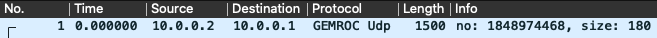
\includegraphics[width=1.0\textwidth]{img/screenshot_col.png}
	\caption{Uzupełniona kolumna protokołu}
	\label{fig:col}
\end{figure}

Po uzupełnieniu podstawowych informacji budowane jest drzewo pakietu. Do drzewa dodawane są kolejne pola pakietu za pomocą
funkcji \texttt{proto\_tree\_add\_*}. Kolejność dodawania obiektów ma wpływ na kolejność wyświetlania. Rozsądnym jest więc
dodawać pola w kolejności ich występowania w pakiecie. Dodatkowym tego atutem jest możliwość zadeklarowania zmiennej offset
i jej zwiększania po każdym przeczytanym polu zgodnie z jego rozmarem. Inaczej konieczne byłoby podawanie pozycji pola jako
stałej wartości przy każdym polu, a w przypadku zmiany specyfikacji protokołu przeliczanie wszystkich wartości.

Dodanie zwykłych obiektów do drzewa dokonywane jest za pomocą funkcji \texttt{proto\_tree\_add\_item()}.
Należy do nich większość typów pól, takich jak liczby całkowite, adresy, ciągi znaków, ale też protokoły.
Dla pól bitowych istnieją specjalne funkcje \texttt{proto\_tree\_add\_bitmask*} Pole bitowe tworzy automatycznie
osobne drzewo, programista nie musi więc tworzyć go jawnie. Konieczne jest za to podanie tablicy pól składających
się na dane pole bitowe. W projekcie są to tablice \texttt{status\_fields} oraz \texttt{data\_fields}.

W funkcji jawnie tworzone są dwa drzewa -- jedno dla całego pakietu, które jest wymagane, oraz jedno dla listy danych.
Umożliwia to jej zwinięcie, co biorąc pod uwagę liczby danych wydaje się być konieczne, oraz organizuje
zawartość pakietu. Utworzenie nowego drzewa możliwe jest tylko na istniejącym już obiekcie. Drzewo dla całego projektu
tworzone jest na protocol\_handle otrzymanym po rejestracji protokołu. Drzewo dla listy danych tworzone jest na dodanym
stringu podpisującym listę. Następnie w pętli dodawane są dane pakietu jako pole bitowe $($bitmask$)$.

Na koniec funkcja dodaje pole dla ilości danych i kończy działanie zwracając ilość zużytych danych.

\subsubsection{Reszta kodu}
W projekcie zaimplementowane są jeszcze dwie funkcje służące do wyświetlania dwóch pól: ASIC id oraz Timestamp ASIC.
Jest to spowodowane tym, że do pierwszego dodana musi być stała 86, a do drugie pole musi być przesunięte (ang. bit shift)
o dwa. Na resztę kodu składają się ponadto deklaracje masek bitowych poszczególnych pól statusu oraz danych, stałych, tabele
elementów pól bitowych, oraz zmienne będące uchwytami dla elementów pakietu.

\subsection{CMake}

Do projektu dołączony jest plik \texttt{CMakeLists.txt}. Większość jego elementów jest stała dla każdej wtyczki opartej o API \texttt{epan}.
Podana jest w nim nazwa projektu, jego wersja, oraz pliki źródłowe potrzebne do kompilacji wtyczki. Plik ten musi zostać zaimportowany
przez inny plik programu \texttt{cmake}. Jest to konieczne, gdyż używa on funkcji pochodzących z kodu projektu Wireshark.

Importowanie odbywa się przez odpowiedni wpis w pliku \texttt{CMakeListsCustom.txt}. Plik ten powinien się znajdować w głównym katalogu kodu źródłowego
programu Wireshark. Jest on jednak opcjonalny, dlatego może zaistnieć potrzeba jego stworzenia. Wzorem winien być wtedy plik \texttt{CMakeListsCustom.txt.example},
w którym należy umieścić względną ścieżkę do katalogu wtyczki. Wtyczka może być traktowana jako wymagana do prawidłowej kompilacji, bądź opcjonalna.
Decyduje o tym umieszczenie jej ścieżki -- jeśli dopisana jest do \texttt{CUSTOM\_PLUGIN\_SRC\_DIR} jej brak skutkuje błędem podczas wykonywania komendy
\texttt{cmake}, jeśli do \texttt{\_OPTIONAL\_CUSTOM\_PLUGIN\_SRC\_DIR} \texttt{cmake} wyświetli tylko informację o niemożności zbudowania wtyczki.

\section{Testy}

Aplikacja testowana była na dwóch zestawach pakietów, zapisanych jako pliki o rozszerzeniu pcap:
\texttt{full.pcap} oraz \texttt{GEM\_ALU1\_ArCO2\_70\_30\_Fe55\_AM\_Th\_55\_HV\_3800\_POS\_8\_part\_015.pcap}.
Wyniki dysekcji drugiego zestawu porównywane były z efektami parsowania pakietów przez narzędzie zewnętrzne,
zapisanymi w pliku \texttt{GEM\_ALU1\_ArCO2\_70\_30\_Fe55\_AM\_Th\_55\_HV\_3800\_POS\_8\_part\_015.txt} oraz
jego rozszerzonej wersji \texttt{GEM\_ALU1\_ArCO2\_70\_30\_Fe55\_AM\_Th\_55\_HV\_3800\_POS\_8\_part\_015\_more.txt}.
z informacją o znaczeniu poszczególnych pól.

\begin{lstlisting}[style=CStyle,caption={Zawartość pliku .txt}]
#RawDataView
#ASIC	Channel	TimeStamp	Adc	PileUp	OverFlow	Gain	Thr	iCal	Trim	TS Asic	TS Fpga
87	24	1948361487724	2012	0	0	249	55	50	23	13676	118918547
87	25	1948361487756	926	0	0	249	55	50	11	13708	118918547
87	26	1948361487700	2153	0	0	249	55	50	13	13652	118918547
88	28	1948361504176	2189	0	0	249	55	50	11	13744	118918548
88	29	1948361504236	1422	0	0	249	55	50	18	13804	118918548
88	30	1948361504188	2107	0	0	249	55	50	17	13756	118918548
88	27	1948361516912	2250	0	0	249	55	50	18	10096	118918549
88	28	1948361516956	1556	0	0	249	55	50	11	10140	118918549
88	29	1948361516964	965	1	0	249	55	50	18	10148	118918549
88	30	1948361516916	2108	0	0	249	55	50	17	10100	118918549
\end{lstlisting}

\begin{table}[H]
	\resizebox{\columnwidth}{!}{
	\begin{tabular}{ |c|c|c|c|c|c|c|c|c|c|c|c| }
		\hline

		ASIC & Channel & TimeStamp & Adc & PileUp & OverFlow & Gain & Thr & iCal & Trim & TS Asic & TS Fpga \\
		\hline
		87 & 24 & 1948361487724 & 2012 & 0 & 0 & 249 & 55 & 50 & 23 & 13676 & 118918547 \\
		87 & 25 & 1948361487756 & 926 & 0 & 0 & 249 & 55 & 50 & 11 & 13708 & 118918547 \\
		87 & 26 & 1948361487700 & 2153 & 0 & 0 & 249 & 55 & 50 & 13 & 13652 & 118918547 \\
		88 & 28 & 1948361504176 & 2189 & 0 & 0 & 249 & 55 & 50 & 11 & 13744 & 118918548 \\
		88 & 29 & 1948361504236 & 1422 & 0 & 0 & 249 & 55 & 50 & 18 & 13804 & 118918548 \\
		88 & 30 & 1948361504188 & 2107 & 0 & 0 & 249 & 55 & 50 & 17 & 13756 & 118918548 \\
		88 & 27 & 1948361516912 & 2250 & 0 & 0 & 249 & 55 & 50 & 18 & 10096 & 118918549 \\
		88 & 28 & 1948361516956 & 1556 & 0 & 0 & 249 & 55 & 50 & 11 & 10140 & 118918549 \\
		88 & 29 & 1948361516964 & 965 & 1 & 0 & 249 & 55 & 50 & 18 & 10148 & 118918549 \\
		88 & 30 & 1948361516916 & 2108 & 0 & 0 & 249 & 55 & 50 & 17 & 10100 & 118918549 \\

		\hline
	\end{tabular}
}

	\caption{Pierwsze 10 rekordów pliku .txt}
	\label{tab:data}

\end{table}

Podczas tworzenia wtyczki autor dążył do zgodności własnych wyników z dostarczonymi,
która finalnie została zapewniona. 

	\begin{figure}[H]
		\centering
			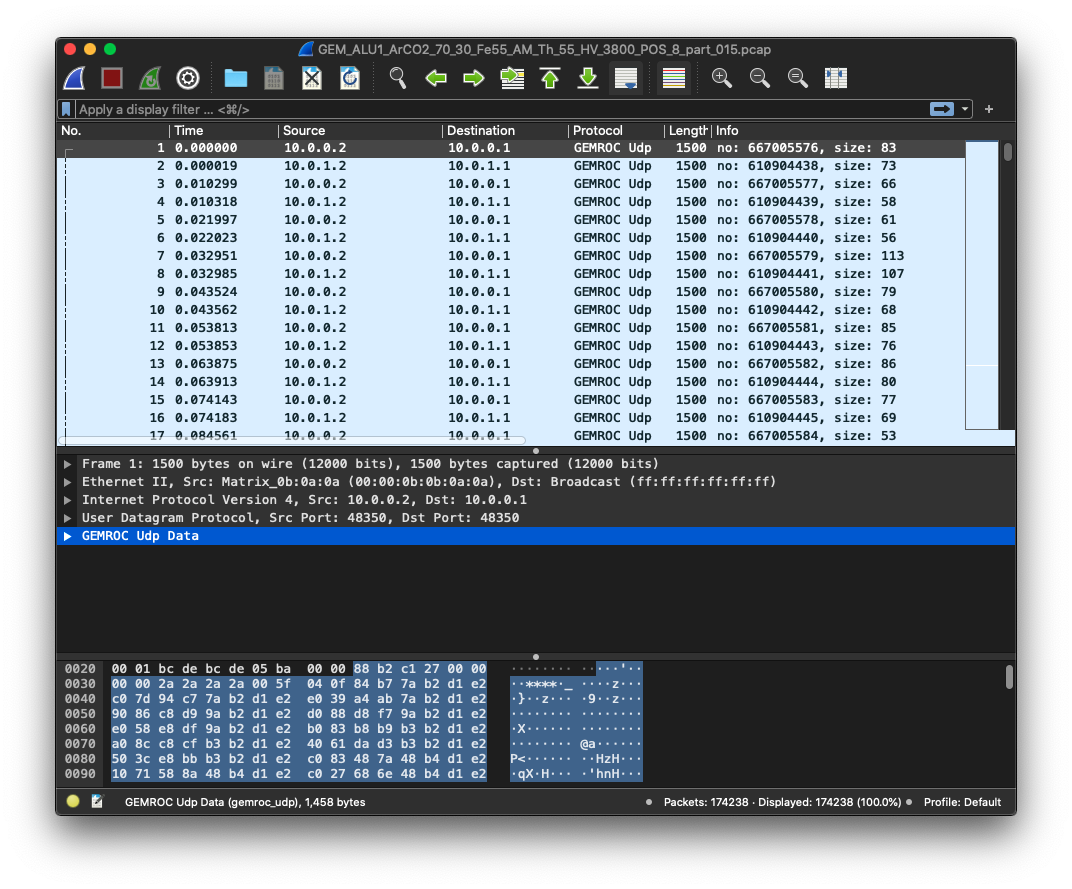
\includegraphics[width=1.0\textwidth]{img/screenshot_dissector.png}
		\caption{Ekran programu Wireshark z wgraną wtyczką}
		\label{fig:dis}
	\end{figure}

Na pierwszym rysunku (Rys. \ref{fig:dis}) wydać efekt dysekcji pakietów z pliku \texttt{GEM\_ALU1\_ArCO2\_70\_30\_Fe55\_AM\_Th\_55\_HV\_3800\_POS\_8\_part\_015.txt}.
W górnej części interfejsu graficznego można zauważyć, że pakiety są poprawnie rozpoznawane i przesyłane do właściwego dekodera, gdyż
kolumny ,,Protocol'' oraz ,,Info'' wypełnione są poprawnie. Plik zawiera dwie zazębiające się transmisje, dlatego co drugi pakiet ma kolejny numer.
Na najniższej pozycji w stosie dekoderów znajduje się protokół GEMROC Udp.

Poniżej widać efekt wczytania tego samego pliku do instalacji programu Wireshark niezawierającej wtyczki. Zamiast Dekodera GEMROC Udp ostatnim poziomem
są surowe dane przesyłane protokołem Udp. Można je przeczytać z najniższego okna programu, lecz wymaga to ręcznego przeliczania wartości pól.

	\begin{figure}[H]
		\centering
			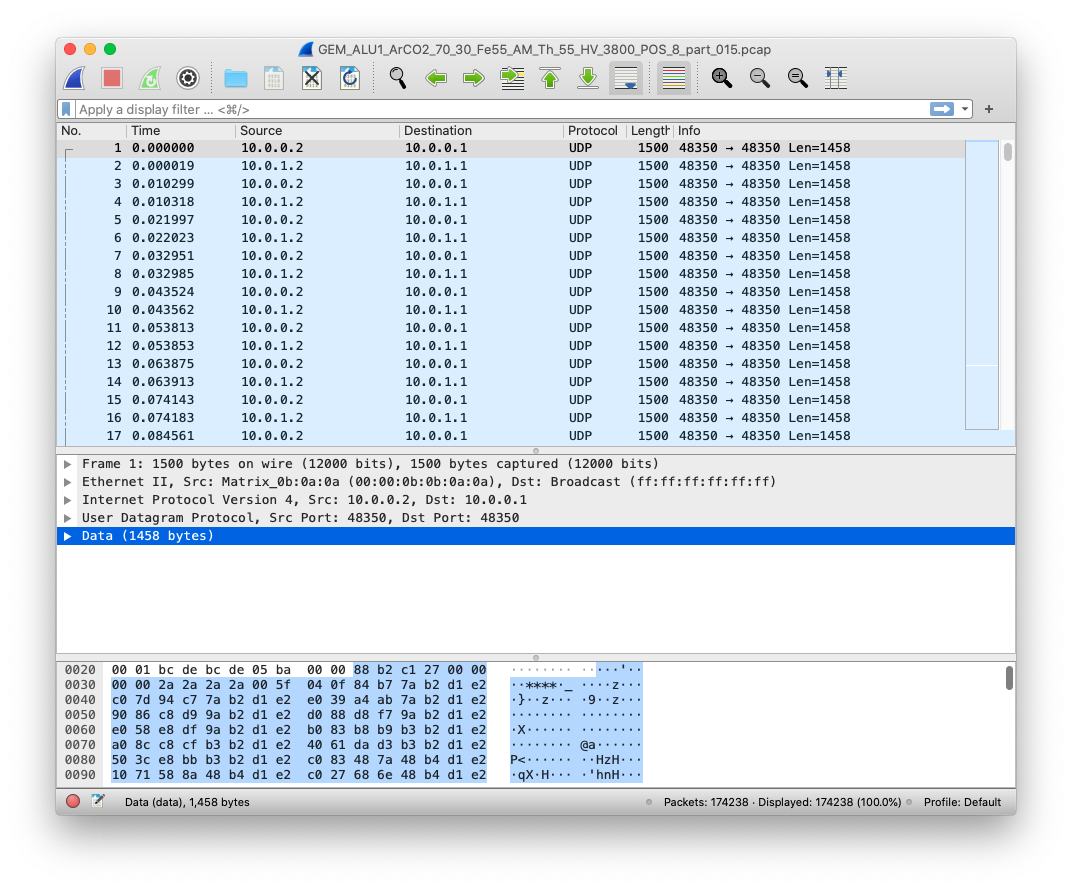
\includegraphics[width=1.0\textwidth]{img/screenshot_no_dissector.png}
		\caption{Ekran programu Wireshark bez wtyczki}
		\label{fig:no_dis}
	\end{figure}



Po rozwinięciu protokołu GEMROC Udp użytkownikowi ukazuje się zawartość pakietu, na którą
składają się 4 pola: ,,Packet no'', ,,Status'', ,,Data list'' oraz ,,Data count''. Zawartość tą widać na poniższym rysunku (Rys. \ref{fig:dis_pack}).

	\begin{figure}[H]
		\centering
			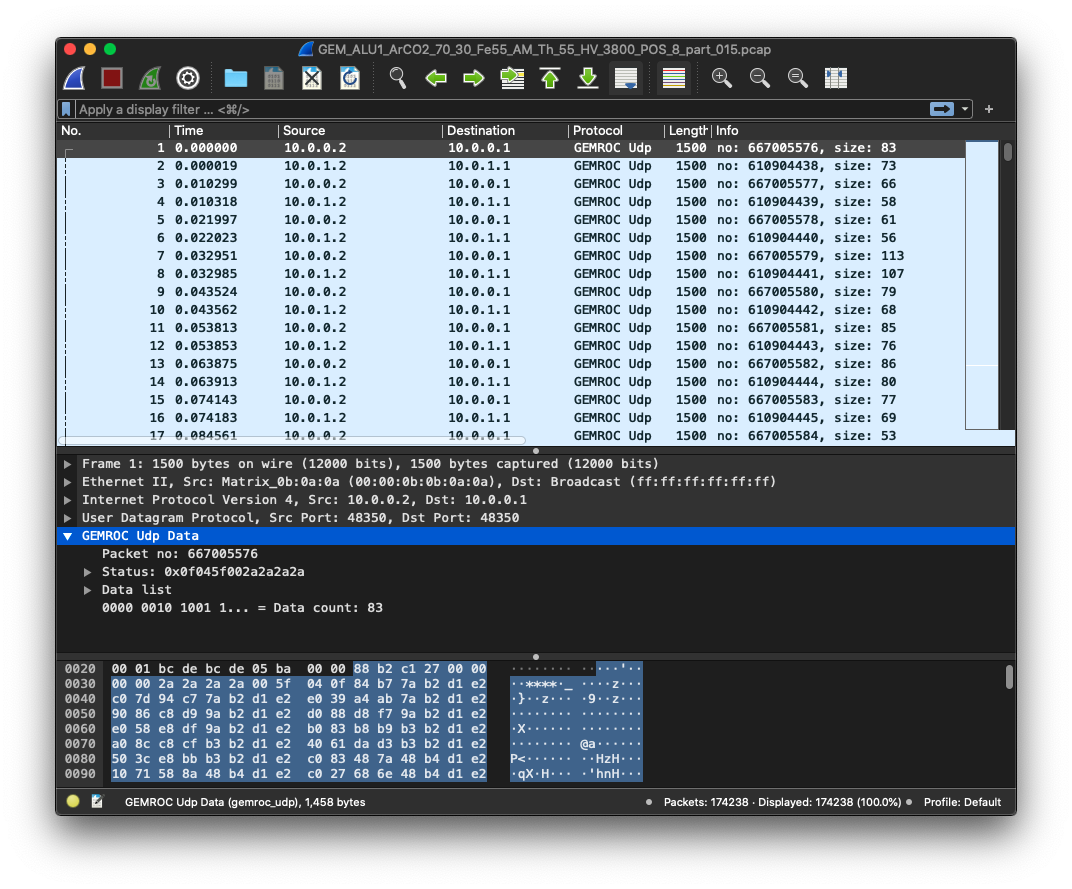
\includegraphics[width=1.0\textwidth]{img/screenshot_dissector_list.png}
		\caption{Zawartość pierwszego pakietu}
		\label{fig:dis_pack}
	\end{figure}

Pierwsze z pól -- ,,Packet no'' -- zawiera wartość zgodną z podaną w skróconym opisie pakietu, zawartym w kolumnie ,,Info''. Kolejne pole -- ,,Status'' --
wyświetla odpowiedni 64-bitowy fragment pakietu w notacji szesnastkowej. Aby poznać szczegółową zawartość konieczne jest jego rozwinięcie (Rys. \ref{fig:dis_status}).

	\begin{figure}[H]
		\centering
			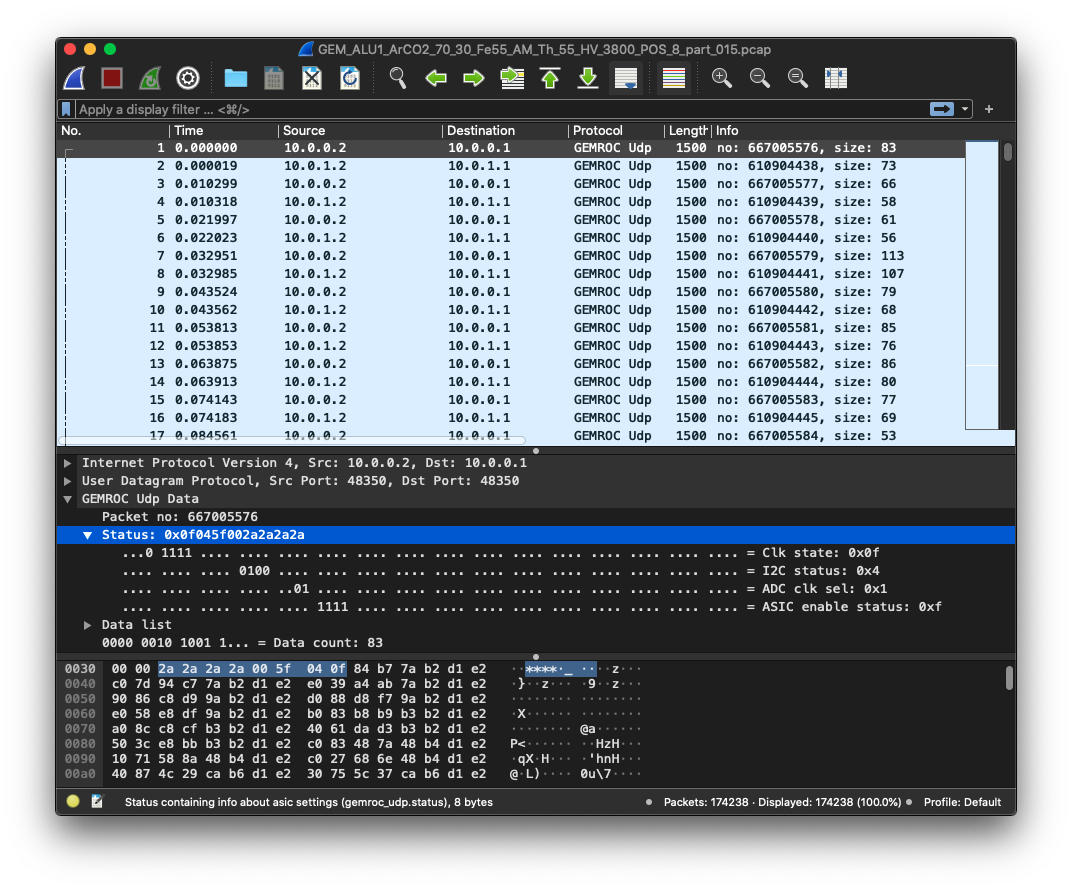
\includegraphics[width=1.0\textwidth]{img/screenshot_dissector_status.png}
		\caption{Zawartość pola ,,Status''}
		\label{fig:dis_status}
	\end{figure}

Pole ,,Status'' zawiera cztery elementy: ,,Clk state'', ,,I2C status'', ,,ADC clk sel'' oraz ,,ASIC enable status''. Dla każdego elementu
pola zaznaczone są wchodzące w jego skład bity. Jest to domyślny sposób wyświetlania wartość pola uzyskiwana jest za pomocą maski.

Kolejnym elementem pakietu jest rozwijana lista danych ,,Data list'' o długości zależnej od zawartości pakietu. Jej rozwinięcie ukazuje
listę ponumerowanych danych (Rys. \ref{fig:dis_data_list}).

	\begin{figure}[H]
		\centering
			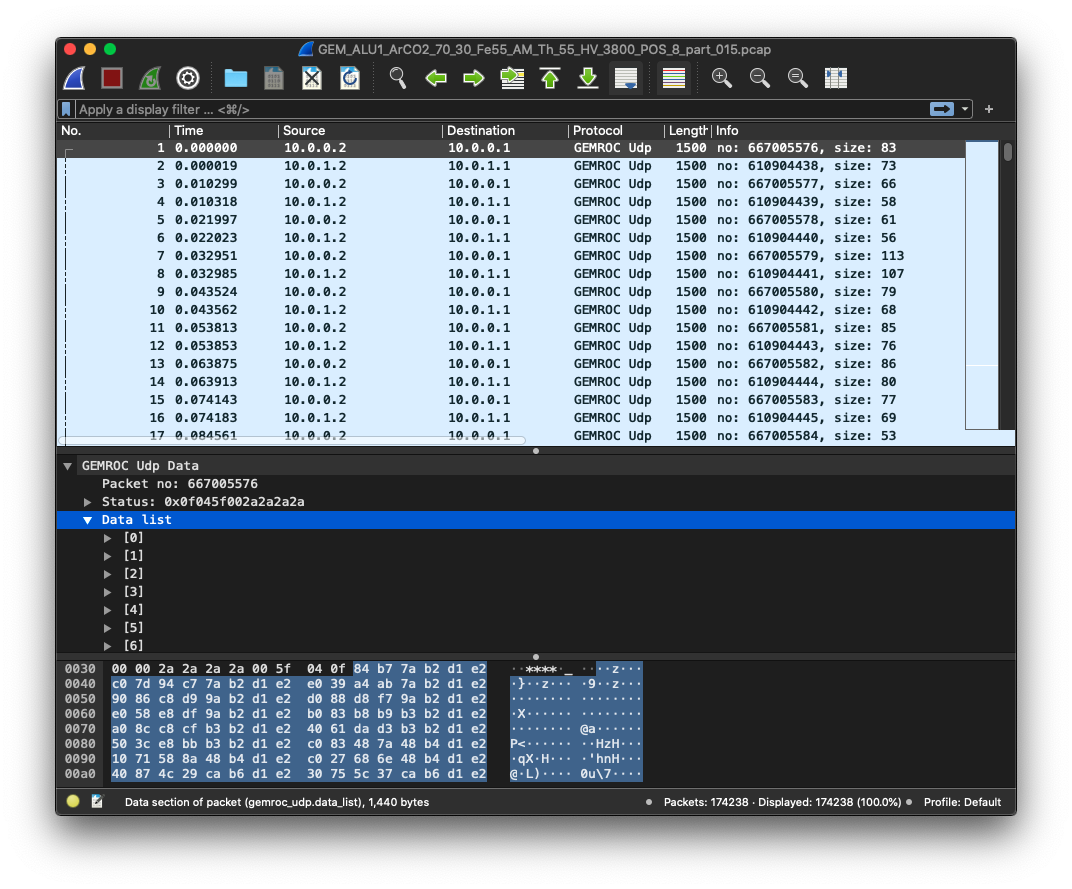
\includegraphics[width=1.0\textwidth]{img/screenshot_dissector_data_list.png}
		\caption{Lista danych pakietu}
		\label{fig:dis_data_list}
	\end{figure}

Dane listy, podobnie jak pole status, są polem bitowym. Każdy element wymaga więc osobnego rozwinięcia. Biorąc pod uwagę średnią długość
listy ułatwia to poruszanie się po niej. Każdy element składa się z pól ,,ADC'', ,,TimeStamp FPGA'', ,,TimeStamp ASIC'', ,,Channel id'', ,,ASIC id'',
,,PileUp'' oraz ,,OverFlow''.

	\begin{figure}[H]
		\centering
			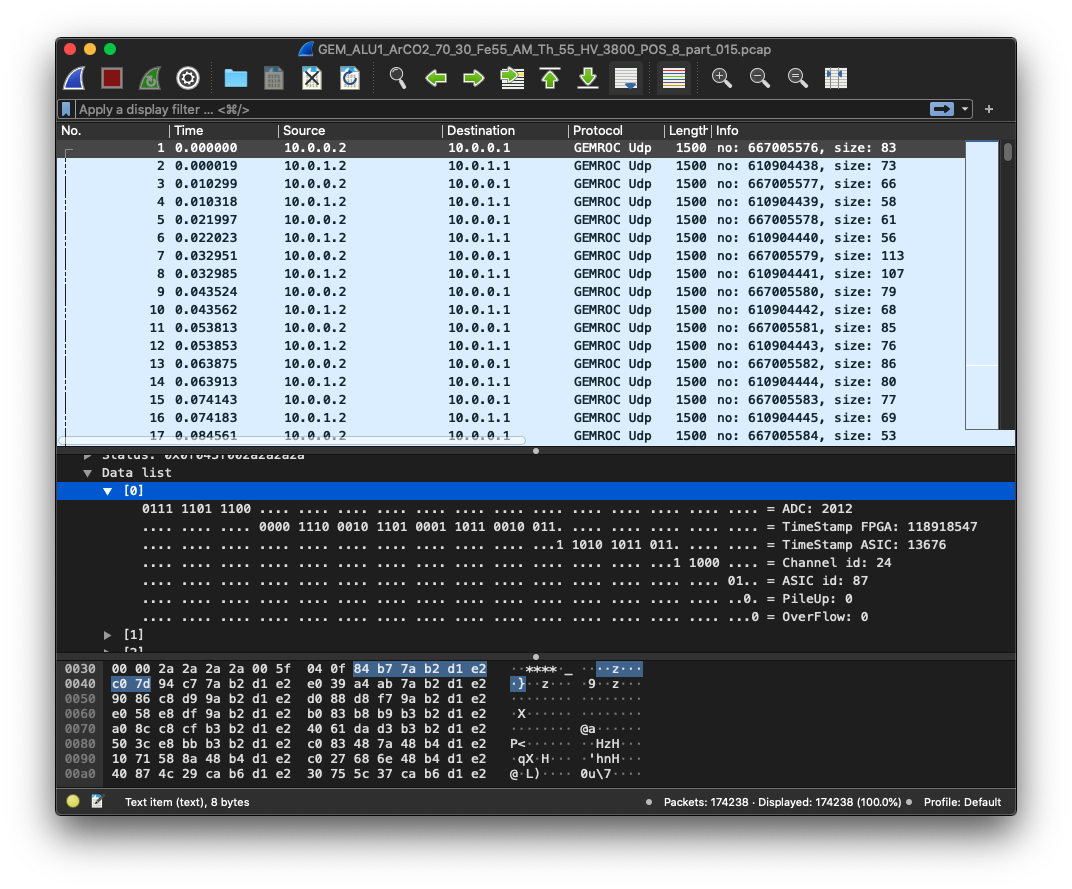
\includegraphics[width=1.0\textwidth]{img/screenshot_dissector_data.png}
		\caption{Dane pakietu}
		\label{fig:dis_data}
	\end{figure}

Dane uzyskane z programu (Rys. \ref{fig:dis_data}) zgodne są z oczekiwanymi wartościami (Tab. \ref{tab:data}).

Ostanim polem pakietu jest ,,Data count''. Zapisane jest one na 13 bitach, użyta została więc maska na liczbie 16-bitowej.
Wartość ta także zgodna jest z oczekiwaniami.

Projekt testowany był również na zestawie danych \texttt{full.pcap}.

\newpage
\section{Podsumowanie}

...




\newpage
\bibliographystyle{srt}
\begin{thebibliography}{99}

	\bibitem{WGDS}
		http://wsgd.free.fr [dostęp: 30.12.2020]


\end{thebibliography}


\vspace{85mm}


\end{document}


